\documentclass{standalone}
\usepackage{tikz}
\usetikzlibrary{decorations.markings}
\begin{document}
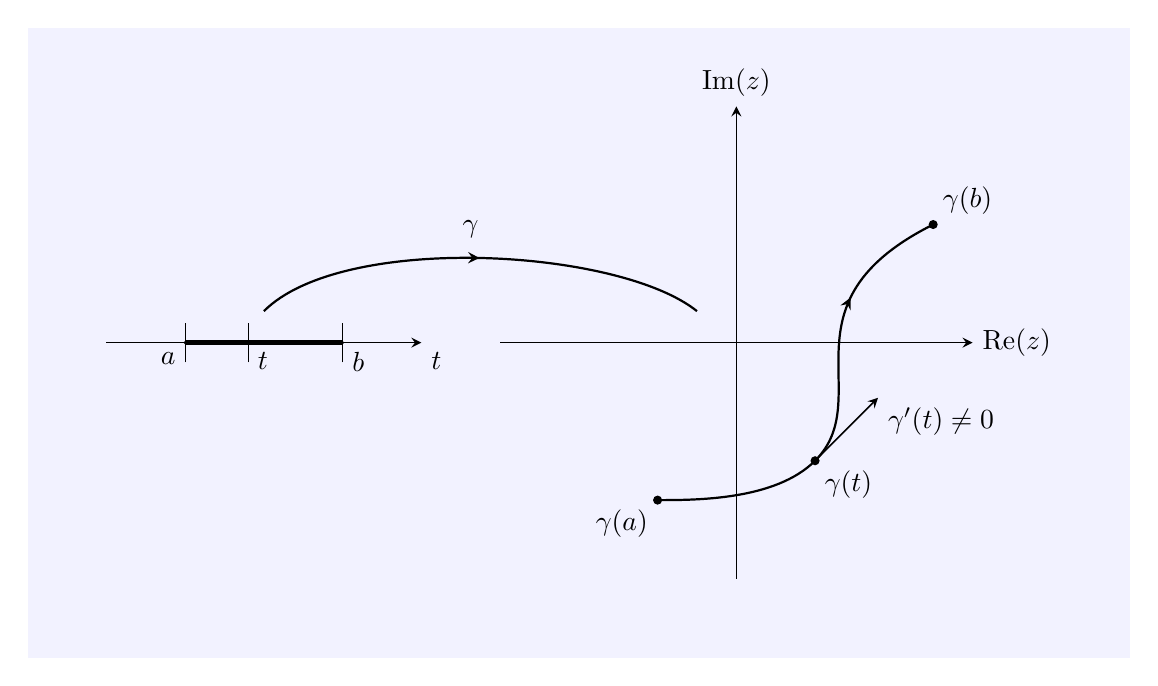
\begin{tikzpicture}
\tikzset{
    every node/.style={font=\normalsize, text=black},
    arrowstyle/.style={->, >=stealth}}
\colorlet{BlueBackground}{blue!5}
% Background for entire canvas
\fill[BlueBackground] (-9,-4) rectangle (5,4);
%Assen
\draw [arrowstyle, semithick](0,-3) -- (0,3) node[above]{$\mathrm{Im}(z)$};
\draw [arrowstyle, semithick](-3,0) -- (3,0) node[right]{$\mathrm{Re}(z)$};
\draw [arrowstyle, semithick](-8,0) -- (-4,0) node[below right]{$t$};
\foreach \x in {-7,-6.2,-5} {
    \draw (\x,-0.25) -- (\x,0.25);
}
\draw[ultra thick] (-7,0)-- (-5,0);
%coordinaten aanduiden op t
\coordinate (a) at (-7,0);
\coordinate (b) at (-5,0);
\coordinate (t) at (-6.2,0);
\draw[fill=black] (a) circle(0.01) node[below left] {$a$};
\draw[fill=black] (b) circle(0.01) node[below right] {$b$};
\draw[fill=black] (t) circle(0.01) node[below right] {$t$};
%coordinaten op C
\coordinate (fa) at (-1,-2);
\coordinate (fb) at (2.5,1.5);
\coordinate (fc) at (1,-1.5);
\draw[fill=black] (fa) circle(0.05) node[below left] {$\gamma(a)$};
\draw[fill=black] (fb) circle(0.05) node[above right] {$\gamma(b)$};
\draw[fill=black] (fc) circle(0.05) node[below right] {$\gamma(t)$};
%gladde kromme er tussen
\draw[postaction={decorate}, decoration={markings,mark=at position 0.75 with {\arrow{stealth}}}]
[black, thick] (fa)
.. controls (-0.5,-2) and (0.5,-2) .. (fc)
.. controls (1.8,-0.7) and (0.5,0.5) .. (2.5,1.5);
\draw [semithick, arrowstyle](fc) -- (1.8,-0.7) node[below right]{$\gamma'(t)\neq0$};
\draw[thick,postaction={decorate}, decoration={markings,mark=at position 0.5 with {\arrow{stealth}}}][black] (-6,0.4)
.. controls (-5,1.4) and (-1.5,1.2) .. (-0.5,0.4);
\node[above right] at (-3.6,1.2) {$\gamma$};
\end{tikzpicture}
\end{document}